%!TEX root = ../elaboration.tex

\chapter{State of the art and related work}
\label{cha:relatedWork}
\epigraph{Many studies carried in the past have focused on subjects related with this work, such as collecting human movement data, human activity recognition and the measuring of game metrics in sports.
    As defined in Section~\ref{sec:objectives}, this work will be about collecting data from basketball players, to analyse it and calculate game metrics, that can be useful to the coaches and to the fans.
    The following sections will present some preliminary concepts fundamental to understand some terms and technologies used later in this work, discuss the related works that served as a starting point to this dissertation and will present some current commercial solutions, used by professional teams.}

%%%%%%%%%%%%%%%%%%%%%%%%
\section{Preliminary Concepts}
This section starts by presenting the available motion sensors, and explaining how they work. After, available communication protocols will be discussed and compared. To finish, different types of IoT computing architectures will be presented.


\subsection{Motion Sensors}
\label{subsec:motion_sensors}
This subsection will present the sensors used to measure motion, in the form of acceleration, rotation, heading or absolute position in the earth. The data sensed by these sensors can then be used and processed to obtain more advanced measures, like velocities, distances or paths.

\subsubsection{Accelerometer}
\label{subsubsec:accelerometer}
Accelerometers measure acceleration forces, which is the rate of change of the velocity of an object, with respect to time. The unit used to acceleration is meter per second squared ($m/s^2$), or G-forces (g). On planet Earth, at sea level, 1 g is equivalent to $9,8 m/s^2$. This value changes slightly with altitude, and will be different on different planets, because of different planet masses.

Accelerometers are useful to measure vibrations, movements and orientation, and can measure static forces, like gravity, or dynamic forces, like moving the sensor.

There are two main ways to measure these forces. Usually accelerometers use capacitive plates, either fixed or attached to springs, and the change of position between these plates changes de capacitance between them. This change is measured and converted into acceleration, as shown in Figure~\ref{fig:acc_cap}. Other way is to use the piezo-electric effect. These accelerometers have microscopic crystal structures can output electrical charge when put under stress, like an acceleration force, as shown in Figure~\ref{fig:acc_piezo}~\cite{accelerometerspark}~\cite{accelerometerde}~\cite{accelerometerglobal}.

\begin{figure}[htbp]
    \centering
    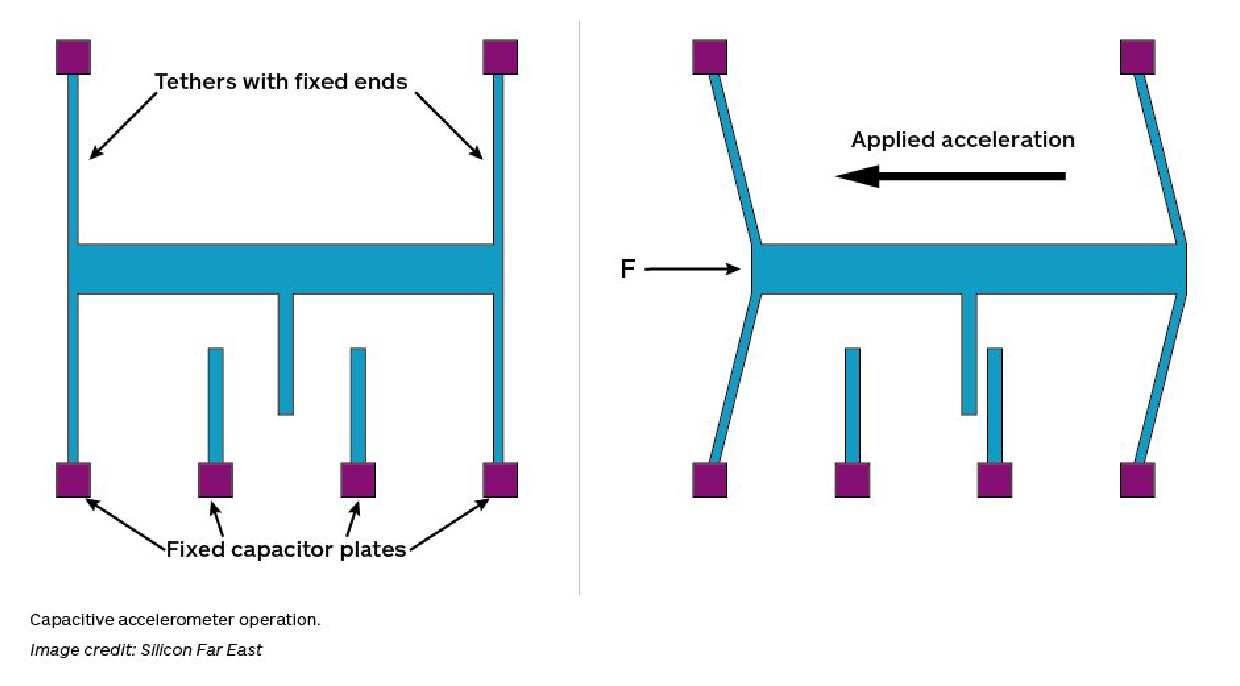
\includegraphics[width=1\linewidth]{accelerometer_cap}
    \caption{Capacitative accelerometer sensor~\cite{accelerometerglobal}}
    \label{fig:acc_cap}
\end{figure}

\begin{figure}[htbp]
    \centering
    \subcaptionbox{Withouth applied force\label{fig:acc_piezo1}}%
    {\includegraphics[width=0.5\linewidth]{accelerometer_piezo_1}}%
    \subcaptionbox{With applied force\label{fig:acc_piezzo2}}%
    {\includegraphics[width=0.5\linewidth]{accelerometer_piezo_2}}%
    \caption{Piezo accelerometer sensor~\cite{accelerometerspark}}
    \label{fig:acc_piezo}
\end{figure}


\subsubsection{Gyroscope}
\label{subsubsec:gyroscope}
Gyroscopes are devices used to measure and maintain orientation and angular velocity.
There are various classes of gyroscopes, used for different needs of performance, cost and volume: mechanical gyroscopes, optical gyroscopes and \gls{MEMS} gyroscopes~\cite{gyro1}.

The most adopted class of gyroscopes for consumer use is the \gls{MEMS} gyroscopes, due to their low cost and low performance. The unit used to measure angular velocity is degrees per second (º/s). \gls{MEMS} gyroscopes usually use a vibrating mechanical element to determine the rate of rotation, in 1, 2 or 3 axes~\cite{gyrospark}.


Most \gls{MEMS} gyroscope take advantage from the Coriolis effect to measure angular velocity. Using a tuning fork configuration, where two masses vibrate constantly in opposite directions, when these masses experience an angular velocity (rotation), the Coriolis force acts on each mass in opposite directions, resulting on a change of capacitance, which is measured to calculate the rate of rotation~\cite{gyromems}. This effect is shown in Figure~\ref{fig:gyro}.

\begin{figure}[htbp]
    \centering
    \includegraphics[width=0.5\linewidth]{gyroscope}
    \caption{Gyroscope sensor~\cite{gyromems}}
    \label{fig:gyro}
\end{figure}

\subsubsection{Magnetometer}
\label{subsubsec:magnetometer}
A magnetometer is a device used to measure the strength and the direction of magnetic fields. The most common method for measuring magnetic fields is using the Hall Effect.  If we have a conductive plate, the electrons would flow from one end to the other. Bringing this plate near to a magnetic field, the electrons would deflect to one side or the other of the plate. Putting a meter between the two sides, the voltage would change accordingly to the direction and strength of the magnetic field, as shown in Figure~\ref{fig:magnetometer}.

This effect can be used to measure the Magnetic North of the Earth, providing handheld devices a sense of orientation in relation to Earth. However, these small magnetometer measurements are easily disturbed by nearby objects, like a computer or a Wi-Fi router, which makes this device unreliable~\cite{magnetometer1}~\cite{magnetometer2}.

\begin{figure}[htbp]
    \centering
    \includegraphics[width=0.5\linewidth]{magnetometer}
    \caption{Magnetometer sensor~\cite{magnetometer1}}
    \label{fig:magnetometer}
\end{figure}

\subsubsection{GNSS}
\label{subsubsec:gnss}
\gls{GNSS} stands for Global Navigation Satellite System, which is a system that provides autonomous geo-spatial, and allows small electronic devices to determine their location precisely. This location is expressed in longitude, latitude and altitude.

There are three \gls{GNSS} systems available for civilian use: Galileo, developed by the Europe Union, \gls{GLONASS}, developed by Russia and \gls{GPS}, developed by the United States of America~\cite{gnss1}. The latter is the most widely used. It was developed to accurately determine the absolute position on Earth, initially for military purposes, but soon was publicly released.

This system is divided into three segments:
\begin{itemize}
    \item Space Segment – 24 satellites orbiting the earth
    \item Control Segment – 5 ground stations positioned on the earth’s equator to control the Space Segment
    \item User Segment – any user that receives the \gls{GPS} signal
\end{itemize}

Triangulation is used to accurately position the user, using at least 4 satellites to obtain position and time correctly, as shown in Figure~\ref{fig:gnss}~\cite{gnss2}.

\begin{figure}[htbp]
    \centering
    \includegraphics[width=0.5\linewidth]{gps}
    \caption{GNSS System~\cite{gnssimg}}
    \label{fig:gnss}
\end{figure}


%%%%%%%%%%%%%%%%%%%%%%%%

\subsection{Communication Protocols}
\label{sec:communication_protocols}
In order to communicate with the sensors, and to collect the data, a communication protocol is needed. In this chapter two widely used communication protocols (Wi-Fi and Bluetooth) are presented. Technologies like Cellular, SigFox, 6LoWPAN, NFC, ZigBee and Z-Wave are not discussed in detail, as they weren't available to be used during this study.

However, all these technologies are compared in the end of this subsection, to realize if the available technologies are the most suitable to fulfill the objectives of this dissertation.

\subsubsection{Wi-Fi}
\label{subsubsec:wifi}
Wi-Fi is a wireless technology that takes advantage of electromagnetic radiation (radio waves), operating in the 2.4GHz and 5 GHz frequencies, to connect mobile computers and network enabled devices like smartphones and IoT devices to local networks and the Internet. The name Wi-Fi is the brand name adopted by the Wi-Fi Alliance~\cite{wifi1}, which holds the Wi-Fi trademark, and certifies products to use this technology.

Wi-Fi technology is based on the Institute of Electrical and Electronics Engineers (IEEE) wireless communication standard 802.11, which has been around for over 20 years, with various different versions of the protocol.
The currently used version is IEEE 802.11ac (Wi-Fi 5), presenting faster and more scalable capabilities than the previous version (802.11n), allowing more bandwidth, faster speeds and lower power usage for each user~\cite{wifi2}.

Regarding IoT, IEEE 802.11 Working Group defined the 802.11ah specification that operates in the sub-1-GHz frequency and supports a greater number of devices per access point, longer transmission range and lower data rate, and is targeted to sensors and IoT applications, competing with Bluetooth technology~\cite{wifi3}~\cite{wifi4}.

\subsubsection{Bluetooth}
\label{subsubsec:bluetooth}
Bluetooth is a low power wireless technology for exchanging data between mobile devices over short distances.

Bluetooth is managed by Bluetooth Special Interest Group, which develops, licenses and holds the trademark. To be able to use Bluetooth, a device manufacturer must meet the Bluetooth SIG standards~\cite{blesig}.

There are two types of Bluetooth technologies:
\begin{itemize}
    \item Basic Rate/Enhanced Data Rate (\gls{BREDR})
    \item Low Energy (\gls{BLE}).
\end{itemize}
While \gls{BREDR} data rates and bandwidth are bigger and support higher data streams like audio streaming, \gls{BLE} has a lower latency and lower power consumption, which is ideal for small IoT devices that only transfer small data packages at a time, as shown in Table~\ref{tab:hla:bluetooth_comparison}~\cite{ble1}.


\begin{table}[ht]
    \caption{Bluetooth Comparison}
    \label{tab:hla:bluetooth_comparison}
    \centering
    \begin{tabular}{lcc}
        \toprule
        \multicolumn{1}{c}{\textbf{Technology}} & \textbf{BR/EDR}     & \textbf{BLE}     \\
        \midrule
        Setup Time                              & 100 ms              & < 6 ms           \\
        Data Rate                               & 125 Kb/s to 2 Mb/s  & 1 Mb/s to 3 Mb/s \\
        Power Consumption                       & 1 (Reference value) & 0.1 to 0.5       \\
        \bottomrule
    \end{tabular}
\end{table}

Bluetooth network topologies can be of different types:
\begin{itemize}
    \item \textbf{Point-to-point (1:1) -} Point-to-point network topology is used for connecting devices one-to-one. In BR/EDR this type of communication is optimized for audio streaming, like headsets, speakers or free-hands systems. In \gls{BLE}, this topology is optimized for data transfer with devices like fitness trackers and PC peripherals.
    \item \textbf{Broadcast (1:m) -} Broadcast establishes one-to-many connections and is only available in \gls{BLE}. This topology is optimized for local information sharing, like point-of-interest information, indoor navigation and asset tracking.
    \item \textbf{Mesh (m:n) -} Mesh establishes many-to-many device connections and is only available in \gls{BLE}. This type of topology is useful when a large number of devices are present and need a trustworthy and safe connection network, like a building with automatic lighting functions or a sensor network. Mesh networks can span a very large physical area. This is particularly useful when a device relies on data from another device that is not in his direct range.
\end{itemize}

These topologies are illustrated in Figure~\ref{fig:bletopologies}.

\begin{figure}[htbp]
    \centering
    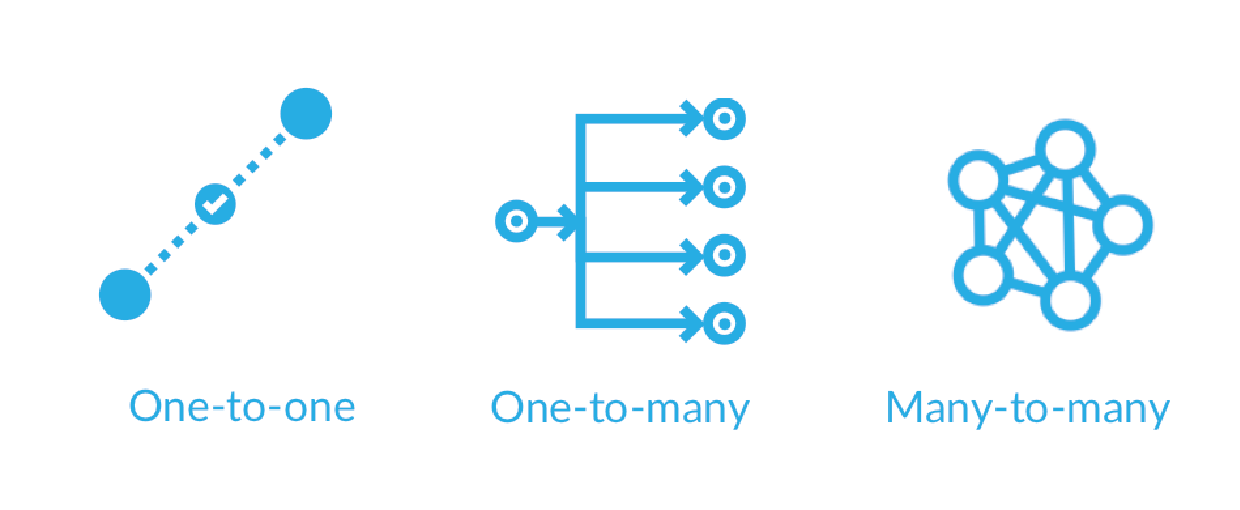
\includegraphics[width=0.8\linewidth]{ble_topologies}
    \caption{BLE Topologies~\cite{ble_mesh_topologies}}
    \label{fig:bletopologies}
\end{figure}


\subsubsection{Communication Protocols Comparison}
\label{subsec:comparison}

Table~\ref{tab:hla:communication_comparison} shows a comparison of the communication protocols mentioned above, regarding the frequency used, the maximum data rate, the range, the power usage and the cost of the technologies~\cite{comparison}.

In order to meet the objective, a low power and low-cost device is needed, with a medium range (enough to cover a basketball court), and a data throughput capable of handling rates of 20-50 Hz.

In terms of cost, Cellular, SigFox, ZigBee and Z-wave are discarded, because they have medium or high costs to be implemented. NFC is also discarded, as it only works in the range of centimeters. 

That leaves us with 6LoWPAN, Wi-Fi and \gls{BLE}. However, for the implementation phase, only Wi-Fi and \gls{BLE} devices are available. These two communication protocols will be tested and implemented, in later stages of this dissertation. 

\begin{table}
    \caption{Communication Protocol comparison}
    \label{tab:hla:communication_comparison}
    \centering
    \resizebox{\textwidth}{!}{%
        \begin{tabular}{lccccc}
            \toprule
            \multicolumn{1}{c}{\textbf{Technology}} & \textbf{Frequency} & \textbf{Max Data Rate} & \textbf{Range} & \textbf{Power Usage} & \textbf{Cost} \\
            \midrule
            Cellular (4G)                           & Cellular Bands     & 100 Mbps               & Several Km     & High                 & High          \\
            SigFox                                  & < 1 GHz            & < 1 kbps               & Several Km     & Low                  & Medium        \\
            6LoWPAN                                 & < 1 GHz            & 250 kbps               & 100 m          & Low                  & Low           \\
            NFC                                     & 13.56 MHz          & 424 kbps               & 10 cm          & Low                  & Low           \\
            ZigBee                                  & 2.4 GHz            & 250 kbps               & 100 m          & Low                  & Medium        \\
            Z-Wave                                  & < 1 GHz            & 100 kbps               & 30 m           & Low                  & Medium        \\
            Wi-Fi                                   & 2.4/5 GHz          & 54 Mbps                & 100 m          & Medium               & Low           \\
            BLE                                     & 2.4 - 2.48 GHz     & 2 Mbps                 & 100 m          & Low                  & Low           \\

            \bottomrule
        \end{tabular}}
\end{table}

\subsection{IoT Computing Architectures}
With the appearance of \gls{IoT}, the computing infrastructure shifted from on-premises servers and software to \textbf{Cloud Computing}. This means that data storage and computation shifted geographically from organization's server rooms to be performed via internet services, in servers owned by the provider of those services~\cite{DZone}.

The advantage of this architectural change frees organization to keep server infrastructures on site, and allows them to have more resources than they could have on premises. It also allows the collection of data from multiple locations and devices, using the internet as a mean of transmitting all the data. The cloud is also capable of performing high performance computing, such as predictive analysis, and have access to a huge amount of data, as the data is also centralized in the cloud~\cite{Inc}.

However, some computing and processing can be brought near to the place where data is produced. \textbf{Fog Computing} and \textbf{Edge Computing} are an extension of cloud computing, only varying in where the location of the computing power is placed.

Fog computing reduces the involvement of the cloud and brings the computation closer to the sensing devices, and improves the use of computation power and reduces the processing time. The fog layer is composed of multiple fog nodes, that receive requests from the \gls{IoT} devices or the end users. 

Edge computing moves computing resources even further close to the end user, and can be described as a more localized version of fog and cloud computing. This paradigm reduces the time it takes to transfer the data from the \gls{IoT} devices to the cloud, and the edge devices can also remove load from the cloud servers and act as \gls{IoT} device managers~\cite{Al-Qamash2018}.

\section{Related work}
\label{sec:relatedWork}
Several authors propose means of transforming data from \gls{IMU} Sensor into meaningful metrics. This section divides the related works in two: first, the related works regarding human activity recognition such as daily activities like walking, climbing stairs and pedestrian tracking will be analysed; then, related works that identify particular basketball activities such as dribbles, passes and shoots are discussed.

\subsection{Human Activity Recognition}
In the area of general human activity recognition, Kerem Altun and Billur Barshan~\cite{Altun2010} propose a method to identify several human activities like sitting, standing, walking, climbing stairs and many other, using data from 5 sensors placed in both legs, both arms and in the chest.
After extracting features and reducing the data, different classification techniques are employed to classify 19 activities. They conclude that Bayesian Decision Making is the best method to identify this type of activities, followed by k-Nearest Neighbor, both performing over 95\%.

Charissa Ann Ronao and Sung-Bae Cho~\cite{Ronao2016} approach the problem of the human activity recognition by proposing a deep convolutional neural network. With data collected from the accelerometer and gyroscope of a smartphone placed in the pocket, they can identify activities walking, sitting and standing, and walking upstairs and downstairs, with a precision of over 94\%.

Hassan \textit{et al.}~\cite{Hassan2018} propose a similar method, also using data from the smartphone's accelerometer and gyroscope, but propose a different classifier. Using a Deep Belief Network, the authors compare their method with other commonly used classification methods, and present better results, with a 95.85\% accuracy.

Regarding pedestrian tracking, Wonho Kang and Youngnam Han~\cite{Kang2015} propose an indoor pedestrian location system using off-the-shelf smartphones. With the embedded accelerometer, gyroscope and magnetometer sensors, they perform step detection, estimate the step length and heading direction to trace the path. The results show a satisfiable tracing of the trajectory of the subject with respect to the ground-truth reference.

Carl Fischer, Poorna Sukumar and Mike Hazas~\cite{Fischer2013} propose a tutorial to implement a pedestrian tracker, using a inertial sensor placed in the foot. By employing techniques like Kalman Filtering to estimate the system error from the measurements of the accelerometer and gyroscope sensors, and Zero-Velocity measurements, they can correct the velocity and position estimates, resulting in a close to ground-truth dead reckoning measurements.

Sebastian Madgwick~\cite{Madgwick} presents an orientation algorithm, using a foot attached \gls{IMU} Sensor, that through dead recognition techniques and correcting the drift of integrating acceleration, when the foot touches the ground, is capable of generating a 3-Dimensional tracing of the foot motion.

\subsection{Basketball Activity Recognition}
N. F. Ghazali \textit{et al.}~\cite{Ghazali2018} compare different machine learning techniques to identify common sport activities like being stationary, walking, running, sprinting and jumping, with data collected from an inertial sensor strapped to the chest. The raw data (accelerometer and gyroscope) was labeled, and features were extracted from this data, filtering the relevant information. Then, 5 different types of classification techniques were employed, and compared between each other. The best classifier achieved an accuracy of 91\%, successfully classifying common sport activities.

Le Nguyen Ngu Nguyen \textit{et al.}~\cite{Nguyen2015} use a multi-sensor system composed by 5 sensors placed in both feet, both legs and in the back. With data collected from the accelerometers, they aim to identify general activities like walking, jogging and running, but also basketball-specific activities like jumpshot, layupshot and pivot. The raw data is firstly preprocessed and segmented, and features are extracted from this data. Then, based on the z-axis acceleration, they separate standing and moving activities. Using a Support-Vector-Machine-based classifier, the moving activities are classified. Although the classifications aren't very accurate, they conclude that more information from the sensors should be used, like the data from the gyroscopes, and that to correctly classify similar activities like dribbling (\textit{i.e.} running with the ball) and running, more sensors should be placed in different body parts (\textit{e.g} on the wrists), to differentiate these activities.

Xiangyi Meng \textit{et al.}~\cite{Meng2018} used the same classification technique, but collected Raw Data from accelerometer and gyroscope sensors, and the sensors were placed in the wrist. The authors only aimed to identify 3 basketball activities: shoots, passes and dribbles. Even though a result of 96\% is achieved for dribbling classification, shoots are easily confused with passes.

Ruijie Ma \textit{et al.}~\cite{Ma2018} uses a wrist mounted \gls{IMU} Sensor in order to identify the posture of basketball player, and recognize nine other basketball movements, such as stand, walk, run, jump, in-situ dribble, dribble while walking, dribble while running, set shot, and jump shot. Using a neural network algorithm to identify this movements, an accuracy of 98.9\% is achieved, but only a subject provided the data for the test and validation phases.

Alexander Holzemann \textit{et al.}~\cite{Holzemann2018} has a similar approach, with wrist-worn \gls{IMU} Sensors, identifiyng activities such as dribbling, shooting, blocking, or passing. Using classifiers, a performance of 84\% is achieved with k-Nearest Neighbor classifier and 88\% with Random Forest classifier, with actions like jump shots performing better than dribbles.

\section{Commercial Solutions}
The most used way of track Basketball players is using video tracking systems. Currently, Second Spectrum is the official optical tracking provider for the \gls{NBA}~\cite{NBAstuffer}. This system uses cameras located around the court to collect 3d spatial data of player and ball location and movements, and play-tracking data like speed, distance, shoots, passes, drives and more~\cite{AWSMe}.

Then, using machine learning algorithms, players and coaches can get detailed reports and insights about player performance. This approach can also be profitable for leagues and media, providing data to interactive applications or using augmented reality video to improve the fan experience.

SportVU is an Optical Tracking system, used by Stats Perform~\cite{StatsPerform}, that with cameras placed around the court and the use of artificial intelligence techniques can gather innovative statistics based on player speed, distance traveled, separation, ball possession and more. They combine the tracking of the player and the ball with historical databases to provide in-depth insights for team and player performances. This optical system is available for basketball and football, and besides providing useful information for team management, this data is also used for fan media, and for betting and fantasy content.

Many other sports use video tracking systems in their games, and they can give very accurate measurements about the players location and team tactics, and even track small movements like shoots and passes in Basketball. However, these systems require high processing power, and are very expensive, being out of reach for minor and amateur teams. Video systems are also attached to the field, and in order to track a team in a different location, the system needs to be installed there. Another drawback is that some video systems don’t work in real-time. They need an operator to tag events, and the processed data is deferred~\cite{VanderKruk2018}.

Other way to track players is using a sensor based approach. Multiple commercial products are used by both amateur and professional teams.

Kinexon~\cite{Kinexon20} developed a player tracking system based on \gls{UWB}. It is comprised of wearable player sensors, that are equipped with 9-axis accelerometer, gyroscope and magnetometer, and an array of base-sensors placed around the court. It can deliver precise 3D-position data, by tracking the players using \gls{RF} technology,  and detects metrics like jumps, sprints, impact, changes of direction, accelerations and deceleration, among many others. It also works both indoors and outdoors.~\cite{WearableTechnologies}.

ShotTracker~\cite{ShotTracker} is tracking system that is made of 3 components: ShotTracker-enabled ball, player sensors and anchors around the court. The Anchors are what locates the players and the ball, and can infer metrics like distances, number of passes, shots and shot types, and have a structured summary of the results of a game. All the data that is collected is analysed and displayed in an application in real-time. The data presented in this application has three targets: the coaches, to improve their team's performance; the players, to analyse and enhance their practice; and the fans, giving them access to advanced team stats and detailed box scores, and even Augmented Reality features to interact with the live game.

STATSports~\cite{STATSports} is a system developed for football player tracking. The players use a pod worn in the back, that is equipped with an accelerometer, a gyroscope, a magnetometer and that collects positional tracking using a GPS device. This device has the ability to calculate internally over 50 metrics in real-time (\textit{e.g.} total distance covered, number of accelerations or decelerations and heart rate), that are then transmitted over a \gls{UWB} network. A cloud-based platform aggregates all the data, and presents available advanced metrics dashboards and individual/group data for players and coaches to consult. It is used widely by several professional football teams.

\section{Chapter summary}
In this chapter we started by analyzing the commonly used motion sensors, the most suitable communication protocols to transmit information in this type of applications and what \gls{IoT} architectures exist, and the pros and cons of each one. With this analysis, it was concluded that 6LoWPAN, Wi-Fi and \gls{BLE} are the most suitable communication protocols to use, but only Wi-Fi and \gls{BLE} will be used in the implementation phase, as they are the only ones available. It was also found that this kind of system could benefit from using an edge-processing style architecture, because it can improve the need to process data in real-time, allowing for low latency computing.

Regarding the related works in this field, the search focused on works that studied human activity recognition in general, identifying activities like sitting, walking, running, jumps and tracking of position, and on works that aimed to classify basketball related activities, like shots, passes and dribbles.

Of the researched works, all of the works found that aimed to classify activity (both human and basketball activities), used machine learning techniques to do so. These techniques, while powerful when trained with large amounts of data, are often used to perform the classification offline, after collecting the data. They are also very resource-intensive. These factors are against the objectives defined for this study. While they are useful to understand what activities and metrics can be classified, other techniques (such as signal analysis and statistics) should be used in the implementation of this system.

In the area of positional tracking, three promising works where found. All revolve around the same concepts: use \gls{IMU} to detect steps, displacement and orientation. The work of Wonho Kang and Youngnam Han~\cite{Kang2015} uses the data collected from a smartphone, with data collected when the smartphone is in the hand, in front of the subject. For basketball players, this is an impossible scenario. The other two works, both used a sensor placed in the foot, which seems like a non intrusive method for collecting data from basketball players. Comparing the two, the work of Carl Fischer, Poorna Sukumar and Mike Hazas~\cite{Fischer2013} seems to produce better overall results, and the details of their work are more detailed. This work will be used later in the implementation of the system prototype.

Regarding the commercial solutions, video-based and sensor-based approaches where analysed. Video systems are discarded, since they don't meet the objectives of this study in terms of cost, performance power and infrastructure. Therefore, that leads us to build a system based on wearable sensors, and so those systems are analysed. 

All the sensor-based systems presented above claim  to be very precise in the metrics they measure, and many of them are used by professional teams in their competitions. However, they all rely on a infrastructure placed in the court, or on external tracking solutions (like \gls{GPS} in the case of STATSports). For Basketball, the use of \gls{GPS} is out of question, as most of the Basketball courts used by amateur teams are indoors. The need of an infrastructure is also not ideal for amateur teams, because it increases the costs and hinders the ability to play in different fields, which are two important factors for amateur teams.

During the development of this work, two companies were contacted. Although we do not have a scenario for it to be possible to calculate a budget, the responses where that the cost of the systems could range between tens to hundreds of thousands of euros, by the time of writing of this dissertation.

The analysis of the state of the art and related work gave us some guidelines: the developed system will use Wi-fi or Bluetooth, as they are the most suitable communication protocols; the system should be built following an edge-computing architecture, to improve the speed of the processing and reduce data transfer latency; and real-time data analysis methods should be used, to provide faster insights on the data collected.